\chapter{Methodology}
\label{chap:methodology}

This chapter outlines the methodology used in this dissertation, including the research design, data sources, preprocessing techniques, model development, and evaluation methods. The objective is to present a clear and reproducible workflow for the analytical process, ensuring the reliability and validity of the findings.

\section{Overview of the Methodology}
\label{sec:overview-methodology}
This dissertation adopts a mixed-methods approach, integrating both quantitative and qualitative research techniques. The quantitative component involves the analysis of large-scale numerical data using machine learning models, while the qualitative component incorporates text analysis techniques applied to unstructured data sources such as policy documents and news articles. This blended approach facilitates a comprehensive understanding of economic trends and policy dynamics.

\section{Data Collection}
\label{sec:data-collection}
Quantitative data was sourced from reputable institutions, including the Government of India, World Bank, IMF, and other international economic databases. Datasets included metrics related to unemployment, inflation, GDP, and fiscal indicators.
For the qualitative component, unstructured textual data was collected from policy documents, ministerial speeches, government press releases, and news articles relevant to economic policy-making. These sources were selected to reflect policy discourse and real-time shifts in governance narratives.

\section{Data Preprocessing}
\label{sec:data-preprocessing}
The numerical datasets underwent preprocessing steps such as handling missing values, normalization, and encoding of categorical variables. These operations were performed using Python libraries such as Pandas and NumPy.
For text data, preprocessing included tokenization, stopword removal, lemmatization, and vectorization. Tools such as NLTK, SpaCy, and Hugging Face tokenizers were employed to prepare textual data for further analysis.

\section{Econometric and Machine Learning Models}
\label{sec:models}
The quantitative analysis employed various econometric models, including Ordinary Least Squares (OLS) regression, Vector Autoregression (VAR), and Granger causality tests. These models were implemented using the Statsmodels library in Python.

For the machine learning component, a range of algorithms were applied, including:

\begin{itemize}
  \item \textbf{Time Series Analysis} -- ARIMA and SARIMA models for forecasting economic indicators.
  \item \textbf{Supervised Learning} -- Linear Regression and Decision Trees for baseline modeling.
  \item \textbf{Deep Learning} -- Recurrent Neural Networks (RNNs) for time series data and Transformers (e.g., BERT) for sentiment analysis.
  \item \textbf{Boosting Models} -- XGBoost and NGBoost for enhanced predictive performance.
\end{itemize}

\subsection{Time Series Analysis}
\label{sec:time-series-analysis}

\subsubsection{ARIMA}
\label{sec:arima}
The Autoregressive Integrated Moving Average (ARIMA) model was used for univariate time series forecasting. ARIMA models are denoted as ARIMA(p, d, q), where $p$ is the order of the autoregressive component, $d$ is the degree of differencing required to make the time series stationary, and $q$ is the order of the moving average component. Parameters were selected based on AIC and BIC scores.

\begin{equation}
  \Delta^d Y_t = \sum_{i=1}^{p} \phi_i \Delta^d Y_{t-i} + \sum_{j=1}^{q} \theta_j \epsilon_{t-j} + \epsilon_t
\end{equation}

\subsubsection{SARIMA}
\label{sec:sarima}
The Seasonal ARIMA model extends ARIMA by incorporating seasonality. SARIMA(p, d, q)(P, D, Q)$_S$ models include additional parameters for seasonal patterns and were selected using cross-validation.

\begin{equation}
  \phi(B) \Phi(B^S) \Delta^d \Delta_S^D Y_t = \theta(B) \Theta(B^S) \epsilon_t
\end{equation}

\subsection{Regression Models}
\label{sec:regression-models}
Regression models are used to establish relationships between dependent and independent variables.

\subsubsection{Linear Regression}
\label{sec:linear-regression}
Linear regression was implemented as a baseline model to predict economic indicators based on historical data. The model assumes a linear relationship between the dependent variable and one or more independent variables.
\begin{equation}
  Y = \beta_0 + \beta_1 X_1 + \beta_2 X_2 + ... + \beta_n X_n + \epsilon
\end{equation}
where $Y$ is the dependent variable, $X_i$ are independent variables, $\beta_i$ are coefficients, and $\epsilon$ is the error term.

\subsubsection{Decision Trees}
\label{sec:decision-trees}
Decision trees were used for regression tasks, providing a non-linear approach to modeling relationships. The model splits the data into subsets based on feature values, creating a tree-like structure.

\begin{equation}
  Y = f(X) = \sum_{i=1}^{n} w_i \cdot I(X \in R_i)
\end{equation}
where $R_i$ are the regions defined by the splits, $w_i$ are the predicted values for each region, and $I(X \in R_i)$ is an indicator function that is 1 if $X$ falls into region $R_i$ and 0 otherwise.

\begin{figure}[H]
  \centering
  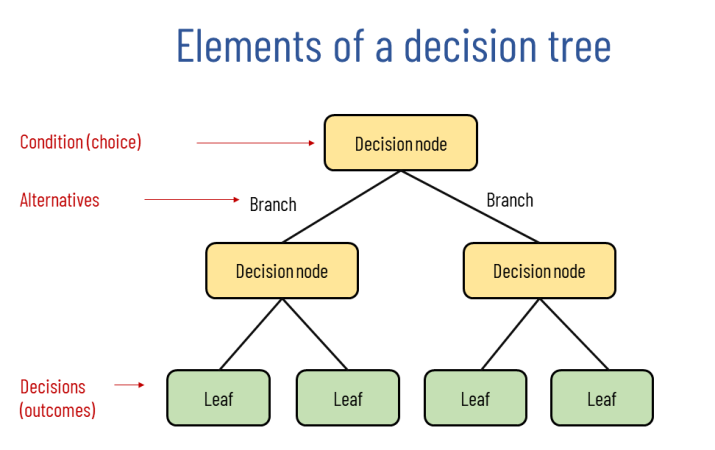
\includegraphics[width=0.5\textwidth]{../images/decision-tree.png}
  \caption{Elements of a Decision Tree}
  \label{fig:decision-tree}
\end{figure}

\subsubsection{Random Forests}
\label{sec:random-forests}
Random forests were employed to improve prediction accuracy by aggregating multiple decision trees. Each tree is trained on a random subset of the data, and the final prediction is the average of all trees.
\begin{equation}
  Y = \frac{1}{T} \sum_{t=1}^{T} f_t(X)
\end{equation}
where $T$ is the number of trees, and $f_t(X)$ is the prediction from tree $t$.

A diagram of a random forest model is shown below:
\begin{figure}[H]
  \centering
  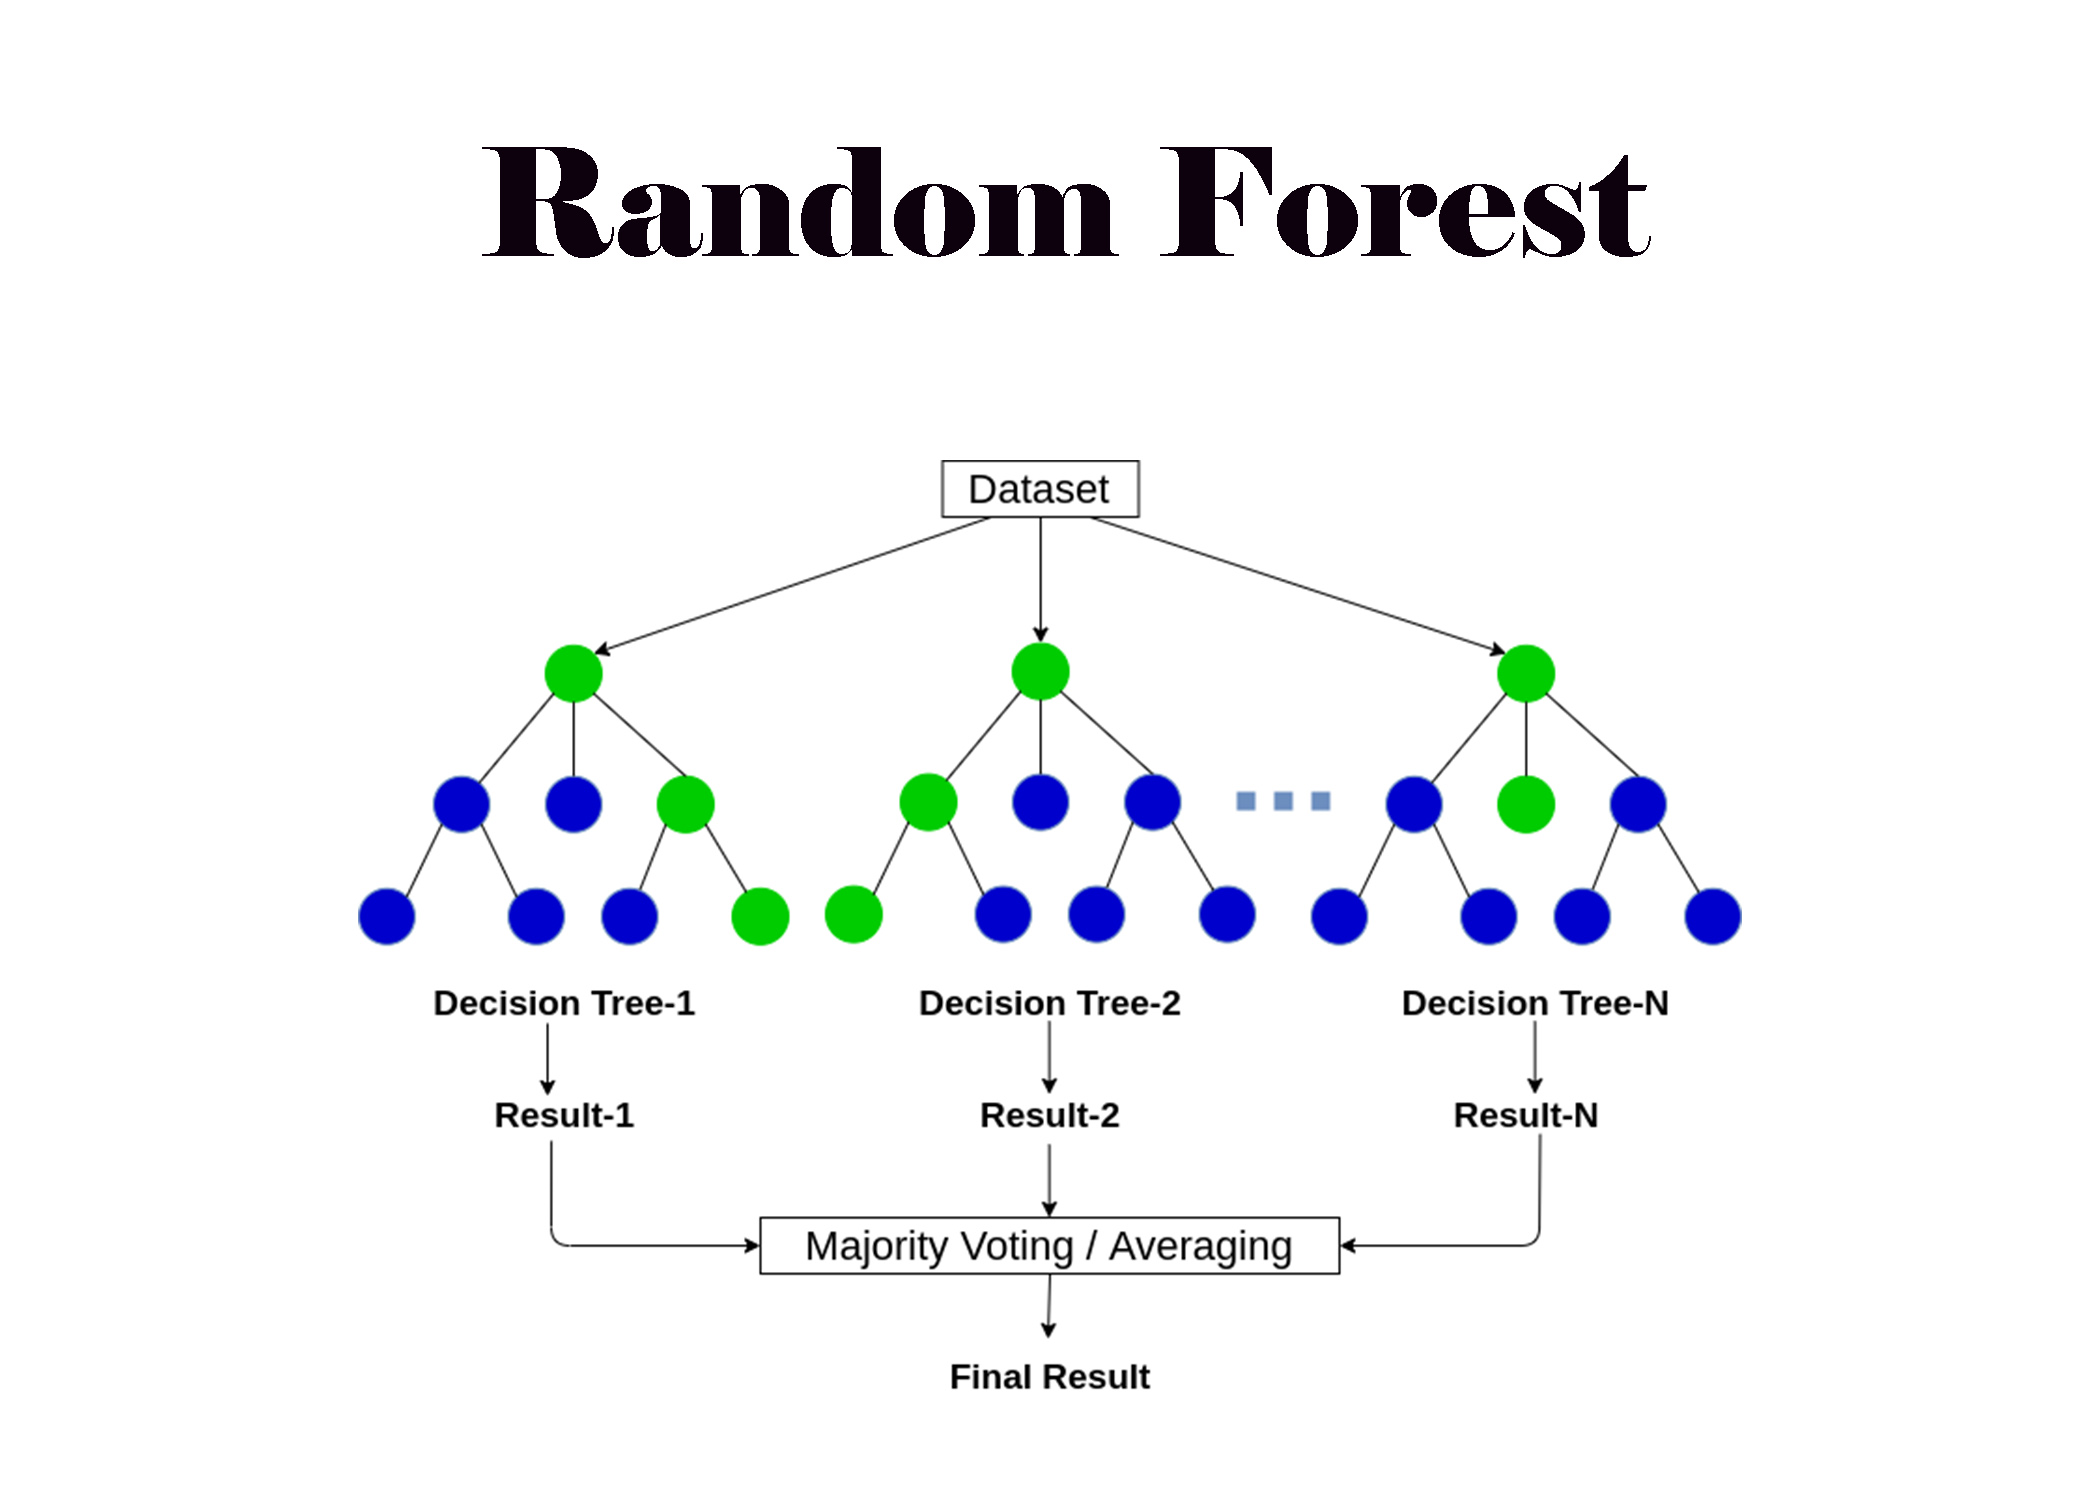
\includegraphics[width=0.5\textwidth]{../images/random-forest.png}
  \caption{Random Forest Model}
  \label{fig:random-forest}
\end{figure}

\subsection{Deep Learning Models}
\label{sec:deep-learning-models}
Deep learning models are based on neural networks and are particularly effective for capturing complex patterns in data. They consist of layers of interconnected nodes (neurons) that process input data and learn to make predictions. They are capable of modeling intricate relationships, making them suitable for tasks such as natural language processing and time series forecasting.

\begin{equation}
  Y = f(W \cdot X + b)
\end{equation}
where $Y$ is the output, $W$ are the weights, $X$ is the input, and $b$ is the bias.

Here is a diagram of a perceptron, the basic and functional unit of a neural network:
\begin{figure}[H]
  \centering
  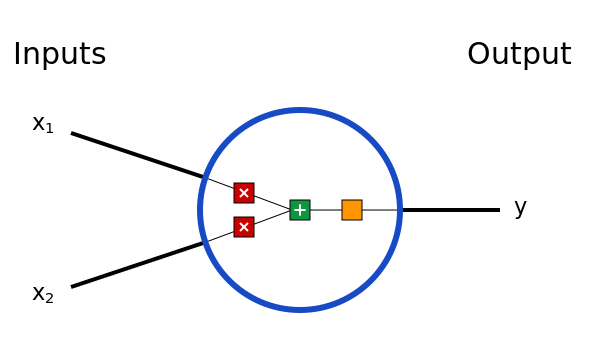
\includegraphics[width=0.5\textwidth]{../images/perceptron.png}
  \caption{Perceptron}
  \label{fig:perceptron}
\end{figure}

Here is a diagram of a simple neural network architecture:
\begin{figure}[H]
  \centering
  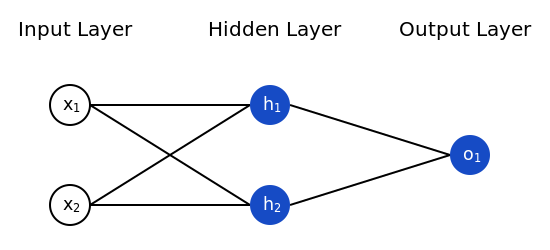
\includegraphics[width=0.5\textwidth]{../images/network.png}
  \caption{Simple Neural Network Architecture}
  \label{fig:neural-network}
\end{figure}

\subsection{Boosting and Hybrid Models}
\label{sec:boosting-hybrid}
To explore ensemble-based forecasting techniques, XGBoost and NGBoost were implemented. XGBoost is a scalable gradient boosting algorithm, while NGBoost enables probabilistic forecasting with confidence intervals.

Hybrid models were also explored by combining structured data (e.g., macroeconomic indicators) with features derived from unstructured data (e.g., sentiment scores from policy speeches). Sentiment scores were calculated using BERT and incorporated as additional features in the boosting models to enhance predictive performance.

\section{Evaluation Metrics}
\label{sec:evaluation-metrics}
Model performance was evaluated using the following metrics:

\begin{itemize}
  \item \textbf{Mean Squared Error (MSE), Root Mean Squared Error (RMSE)} -- for regression and time series models.
  \item \textbf{Accuracy, Precision, Recall, F1-Score} -- for classification tasks.
  \item \textbf{Negative Log-Likelihood (NLL)} -- for probabilistic models like NGBoost.
\end{itemize}

These metrics were computed using Scikit-learn and Statsmodels libraries.

\section{Tools and Frameworks}
\label{sec:tools-frameworks}
All implementations were carried out using Python in the Jupyter Notebook environment. Key libraries included Pandas, NumPy, Matplotlib, Scikit-learn, Statsmodels, PyTorch, and Hugging Face Transformers. NLP tasks employed NLTK, SpaCy, and Gensim for preprocessing and sentiment extraction.

This toolset enabled a comprehensive, modular, and reproducible workflow for analyzing and forecasting economic indicators using both structured and unstructured data.